\section{Convoluzione}

\begin{quote}
	\emph{In matematica, in particolare nell'analisi funzionale, la convoluzione è un'operazione tra due funzioni di una variabile che consiste nell'integrare il prodotto tra la prima e la seconda traslata di un certo valore. }
\end{quote}
\hspace*{\fill} \href{https://it.wikipedia.org/wiki/Convoluzione}{-Wikipedia}.

\subsection{Convoluzione lineare e discreta}

L'operazione di convoluzione tra funzioni continue è definita in tale modo:
\begin{equation}
	f \circledast g = \int^{\infty}_{- \infty} f(\tau)g(t-\tau)d\tau = \int^{\infty}_{- \infty} f(t - \tau)g(\tau)d\tau
\end{equation} \label{eq:conv_lineare}

La convoluzione discreta, invece, è definita come:
\begin{equation}
	\sum^{\infty}_{m= - \infty} f[m]g[n-m] = \sum^{\infty}_{m= - \infty} f[n-m]g[m] 
\end{equation} \label{eq:conv_discreta}

\subsection{Convoluzione circolare}
Data una funzione $x_T$ di periodo $T$, la sua convoluzione con una funzione $h$ è ancora periodica, si dice convoluzione circolare e si calcola nel seguente modo:

\begin{equation}
	(x_T \circledast h)(t) = \int^{ \infty }_{- \infty} h( \tau ) \cdot x_T (t - \tau ) d \tau =  \int^{ t_0 + T}_{t_0} h_T ( \tau ) \cdot x_T(t - \tau ) d \tau
\end{equation}

Dove $t_0$ è arbitrario e $h_T$ è espresso come:

\begin{equation}
	h_T(t) = \sum^{\infty}_{k= - \infty} h(t-kT)
\end{equation}

Data una funzione $g_N$ periodica con periodo $N$, la sua convoluzione discreta è calcolata come:

\begin{equation}
	\label{eq:conv_circ_disc}
	(f \circledast g_N)[n] = \sum^{N-1}_{m=0} f[m]g[(n-m)_{mod N}]
\end{equation}




\section{Esercizio 1: Convoluzione lineare}
Il testo dell'esercizio chiede di eseguire la convoluzione tra le seguenti funzioni:

\begin{equation}
	\label{eq:x1_lab1}
	x(n) = \begin{cases} 
	sin(\frac{\pi n}{5}) & \mbox{se }  0 \le n \le 4 \\ 
	0 & \mbox{altrove} 
	\end{cases}
\end{equation} 

\begin{equation}
	\label{eq:y1_lab1}
	y(n) = \begin{cases}
	1 & \mbox{se } 0 \le n \le 2 \\
	0 & altrove	
	\end{cases}
\end{equation}

Senza l'ausilio del comando di libreria di MATLAB: \textit{conv()}. Per farlo è necessario applicare loro la formula per la convoluzione discreta (\ref{eq:conv_discreta}) "manualmente". Procediamo quindi alla scrittura del codice per passi:

\begin{enumerate}

	\item Creazione dei due vettori sui quali applicare la convoluzione. (\textit{x} ed \textit{y}).
	\item Definizione della lunghezza finale che deve avere il vettore finale e adattamento del vettore x per la lunghezza ricercata.
	\item Iterazione con doppio ciclo \textit{for} per ottenere il risultato.
	
\end{enumerate}

\begin{figure}[H]
\centering
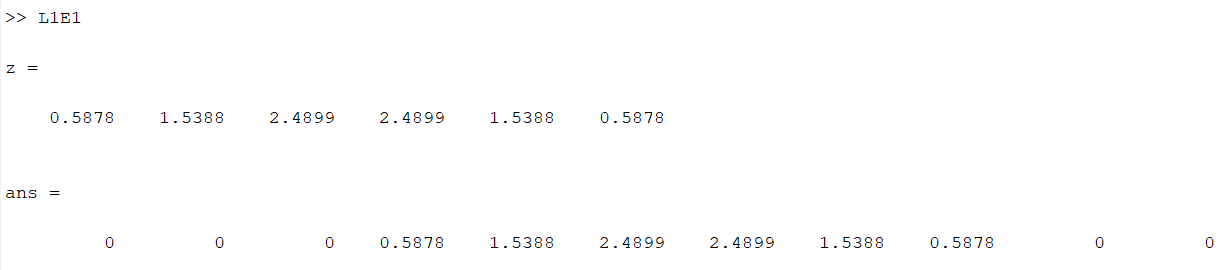
\includegraphics[width=\textwidth]{./images/cap2/convoluzione_es1.png}
\caption{Risultato del codice (z), confrontato con la funzione di libreria \textit{conv()}.}
\label{fig:convoluzione_es1}
\end{figure}

I risultati in figura \ref{fig:convoluzione_es1} differiscono per dimensione solo per l'implementazione della funzione di MATLAB, ma i valori non nulli sono gli stessi.

\section{Esercizio 2: Convoluzione circolare}
Prendendo sempre in considerazione la funzione \ref{eq:x1_lab1} e la \ref{eq:y1_lab1}, l'esercizio è similare al precedente e prevede che venga calcolata la convoluzione circolare tra i due segnali senza ricorrere alla funzione di libreria \textit{cconv()}.
\par
Per fare ciò è necessario allocare e dimensionare adeguatamente un vettore z di zeri di dimensione \textit{a}, che è il massimo tra la lunghezza di \textit{x} e \textit{y}. Ciò dipende dal fatto che la convoluzione circolare contiene un numero di campioni pari a tale valore. Fatto ciò è possibile procedere al calcolo in maniera iterativa della convoluzione circolare fra i due segnali riportando gli indici in base 0 e utilizzando la funzione libreria \textit{mod()}.

\begin{figure}[H]
\centering
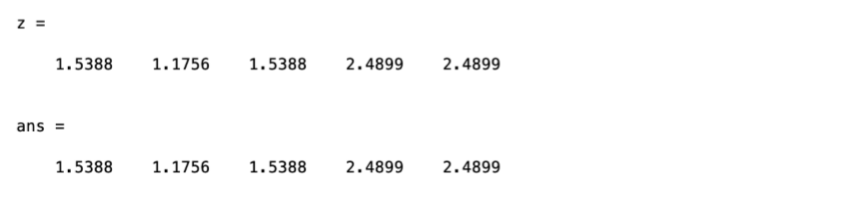
\includegraphics[width=\textwidth]{./images/cap2/convoluzione_es2.png}
\caption{Output dell'esercizio 2.}
\label{fig:convoluzione_es2}
\end{figure}

Il risultato, ottenuto tramite il processo iterativo del codice, che traduce in linguaggio MATLAB la \ref{eq:conv_circ_disc}, fornisce gli stessi valori della funzione di libreria, come si vede in figura \ref{fig:convoluzione_es2}.

\section{Esercizio 3: Mutua correlazione e stima del ritardo}
\begin{quote}
	Un segnale \textit{x(n)} di durata \textit{N} campioni viene irradiato periodicamente dall'antenna di un trasmettitore. Un ricevitore mobile (che conosce il segnale \textit{x(n)}) riceve una versione rumorosa e ritardata del segnale trasmesso.
\end{quote}

\begin{equation}
	r(n)=x(nD) + g(n)
\end{equation}

Dove D è un valore di ritardo (intero) e \textit{g(n)} è un segnale di rumore additivo gaussiano bianco con varianza $\sigma^2$.
\par
Si procede all'implementazione in MATLAB della funzione \textit{mychannel()}:

\begin{figure}[H]
\centering
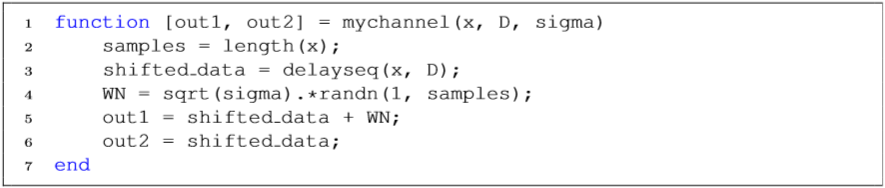
\includegraphics[width=\textwidth]{./images/cap2/mychannel_impl.png}
\caption{Implementazione della funzione mychannel. }
\end{figure}

In seguito è possibile produrre un grafico della stima del ritardo D per diversi valori di \textit{N} e $\sigma^2$ sia nel caso in cui \textit{configBit} (presente in Esercitazione13.m) corrisponde a 0 e 1.
\\

$N = 1000;  \sigma^2= 5$

\begin{minipage}{.45\textwidth}

	\begin{figure}[H]
		\centering
		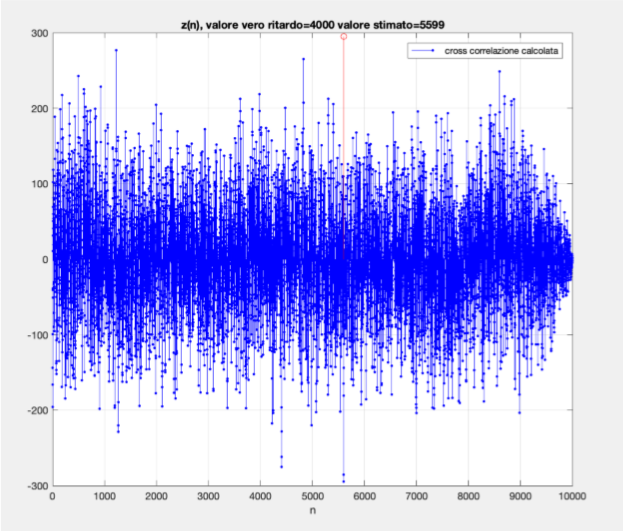
\includegraphics[width=\textwidth]{./images/cap2/es3_grafico1.png}
	\end{figure}
	
\end{minipage}
\hfill
\begin{minipage}{.45\textwidth}
	
	\begin{figure}[H]
		\centering
		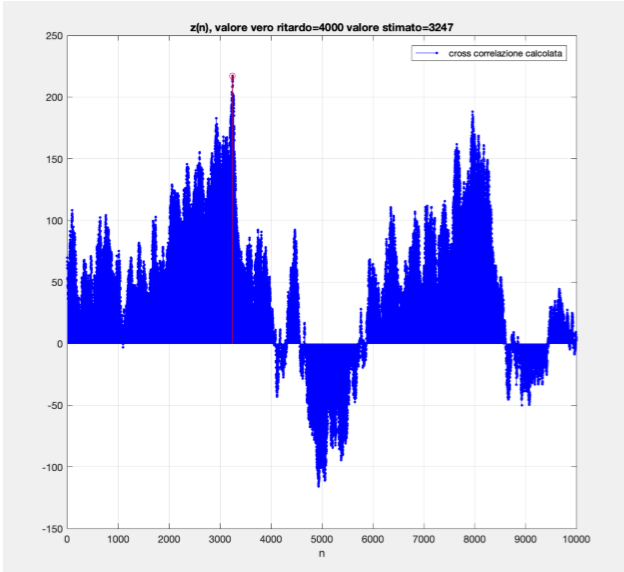
\includegraphics[width=\textwidth]{./images/cap2/es3_grafico2.png}
	\end{figure}

\end{minipage}

\bigskip

$N = 15000; \sigma^2 = 10$

\begin{minipage}{.45\textwidth}
	
	\begin{figure}[H]
		\centering
		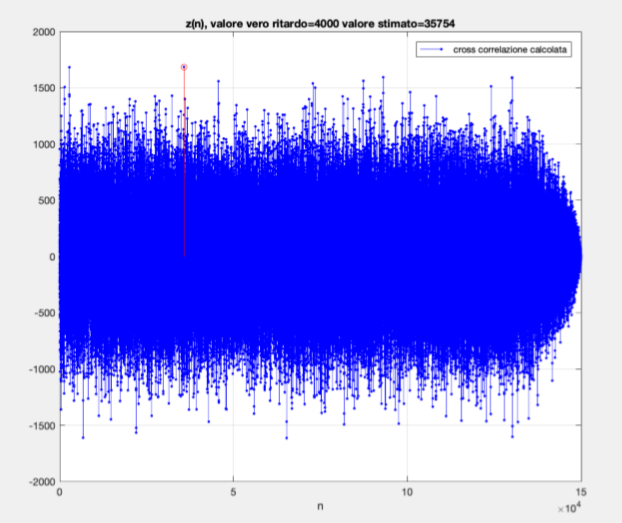
\includegraphics[width=\textwidth]{./images/cap2/es3_grafico3.png}
	\end{figure}	
	
\end{minipage}
\hfill
\begin{minipage}{.45\textwidth}

	\begin{figure}[H]
		\centering
		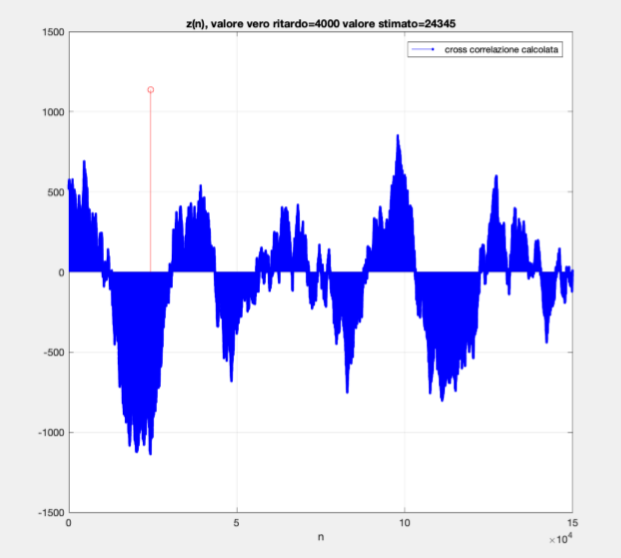
\includegraphics[width=\textwidth]{./images/cap2/es3_grafico4.png}
	\end{figure}

\end{minipage}